% ----------------------------------------------------------
% Teoria
% ----------------------------------------------------------
\chapter{Teoria}
\label{chap:teoria}

O trabalho desenvolvido nesta tese tem como base métodos de
solução numérica de equações diferenciais parciais. Neste capítulo, são
apresentadas as bases teóricas da modelagem matemática
dos problemas e dos métodos de solução utilizados.

%, bem como uma
%breve descrição da física por trás do funcionamento de reatores
%nucleares.

%\begin{figure}[htb]
%  \caption{Teoria: o sistema acoplado.}
%  \centering\includegraphics[scale=0.7]{figuras/teoria1.png}
%  \label{metodoetapas}
%  \legend{Fonte: autor}
%\end{figure}

% **********************************************
\section{Termo-hidráulica}
\label{sec:th}

A Termo-hidráulica é a área de estudo dos de transferência
de calor e massa, processos fluido-mecânicos com transporte de energia e
massa em sistemas nucleares. Os principais fenômenos estudados incluem condução,
convecção, transferência de calor por radiação, mudanças de fase e escoamentos
monofásicos e multifásicos.

A análise termo-hidráulica de sistemas de conversão de energia envolve a solução
das equações de transporte de massa, momento e energia \cite{Todreas2012}. Nesta
tese, a análise deste tipo de sistema é feita utilizando-se o a mecânica
de fluidos computacional (CFD). O CFD é, grosso modo, uma forma de se resolver
problemas físicos complexos pelo uso de métodos numéricos em sistemas
computacionais. Tais métodos numéricos, funcionam descrevendo equações diferenciais
definidas em domínios contínuos em sistemas de equações algébricas, de modo que
sejam resolvidos numericamente. Para transformar o sistema contínuo num sistema
discreto o domínio contínuo é discretizado em um conjunto de subdomínios menores
e conectados que formam uma malha de pequenos elementos (volumes ou células), Figura \ref{fig:dom},
para os quais a solução discreta pode ser obtida \cite{dosSantos2012}.

\begin{figure}[htb]
  \caption[Domínio contínuo e discretizado.]{Domínio contínuo (à esquerda) e discretizado (à direita).}
  \centering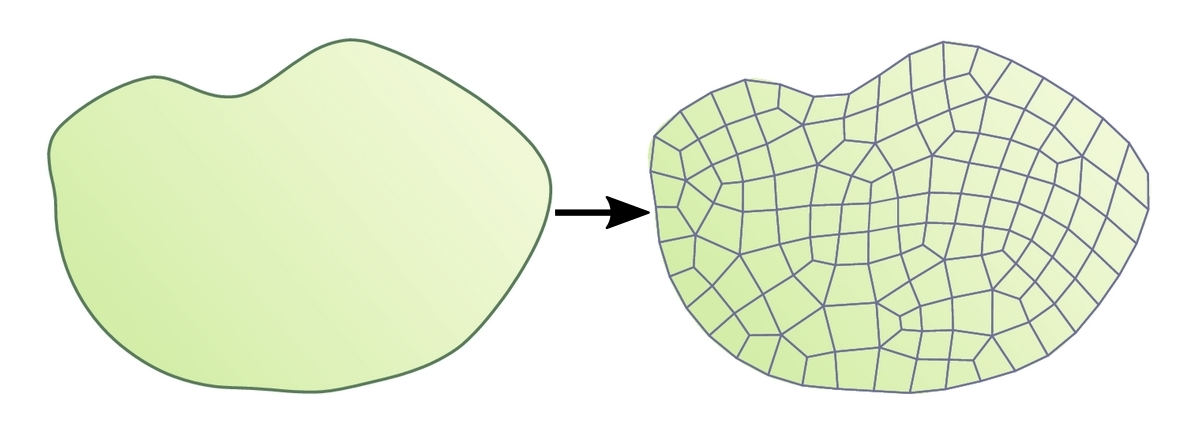
\includegraphics[scale=1.3]{figuras/dom.png}
  \label{fig:dom}
  \legend{Fonte: \cite{Theler2013b}}
\end{figure}

A análise por CFD envolve, geralmente, 5 etapas distintas:

\begin{itemize}
\item Modelagem matemática: Equivale a definir, com base no conhecimento
  físico do problema, as hipóteses válidas, eventuais simplificações e
  seus impactos na solução final. A partir das definições, é necessário
  descrever as condições iniciais e de contorno de problema, as propriedades
  termo-físicas, químicas, fenômenos modelados e quaisquer outras características
  necessárias à solução do problema.
\item Geração da malha: A partir da geometria do sistema, que equivale ao
  domínio contínuo, é necessário gerar uma malha. Essa malha pode ser refinada
  em pontos estratégicos, ser estruturada ou não-estruturada e possuir elementos
  de diferentes formatos. A malha utilizada na solução de um problema tem impacto
  direto no tempo de simulação, na qualidade da solução e até mesmo no alcance
  da solução. Em um projeto de CFD, aproximadamente 50\% do tempo é dedicado a geração
  da geometria e da malha \cite{Versteeg2007}.
\item Solução: Nesta etapa são resolvidos os sistemas lineares obtidos pela
  discretização do domínio.
\end{itemize}
%Nesta seção serão apresentadas
%as equações utilizadas na modelagem de um sistema termo-hidráulico monofásico e
%estacionário.

% **********************************************
%\subsection{Equações governantes}
%\label{subsec:eq}


% **********************************************
%\subsubsection{Fluidos}
%\label{ssubsec:fluid}

% **********************************************
\subsection{Turbulência}
\label{subsec:}

% **********************************************
\subsection{Modelo termo-hidráulico discretizado}
\label{subsec:modeloth}


% **********************************************
%\subsubsection{Sólidos}
%\label{ssubsec:solid}

% **********************************************
\section{Neutrônica}
\label{sec:neutronica}

Neutrônica pode ser definida como o estudo do movimento e interações dos nêutrons
com a matéria. O conhecimento de neutrônica é fundamental para determinar o
comportamento de um reator nuclear ou outros elementos que utilizem nêutrons
em feixes. A neutrônica é, em última instância, o estudo do transporte de nêutrons.

A probabilidade de interação entre um nêutron incidente e um núcleo alvo é caracterizada
pela seção de choque microscópica (unidade \textit{barn}, símbolo $\sigma$ e
equivalente a $10^{-24} cm^2$), que depende do núcleo alvo, do tipo de interação e da
energia do nêutron incidente. Essa dependência pode ser complicada devido a diversos fatores,
como a ordem de grandeza das energias envolvidas, levando a variações súbitas nas probabilidades
de interação. Estas variações são chamadas ressonâncias. A seção de choque macroscópica nada mais
é do que a seção de choque microscópica multiplicada pela densidade nuclear. Ela dá as probabilidades
médias de reação entre nêutrons de determinada energia com o material presente considerando a massa
do material. Sua unidade é dada em $cm^{-1}$.

%No escopo desta tese, é suficiente afirmar que as seções de choque são elementos fundamentais
%na descrição e, portanto, no cálculo neutrônico. 

% **********************************************
\subsection{Dados nucleares}
\label{subsec:dn}

% **********************************************
\subsection{Métodos estocásticos}
\label{subsec:mc}

% **********************************************
\subsection{Métodos determinísticos}
\label{subsec:det}

% **********************************************
\subsubsection{Equação de Transporte}
\label{ssubsec:transp}

% **********************************************
\subsubsection{Aproximação por Difusão}
\label{ssubsec:difusao}

% **********************************************
\subsection{Modelo neutrônico discretizado}
\label{subsec:modelon}
